\subsection{Training Evaluation}
To evaluate the training progression of our optimized QLSTM model, we monitor the mean loss across all stocks with respect to the number of epochs. Each epoch represents a complete training cycle on the entire stock dataset, which promotes model generalization and decreases the potential for overfitting to a single stock. This approach ensures that the model's learning is robust and applicable across diverse stock behaviors.

\begin{figure}[!htbp]
  \centering
  \scalebox{0.30}{
  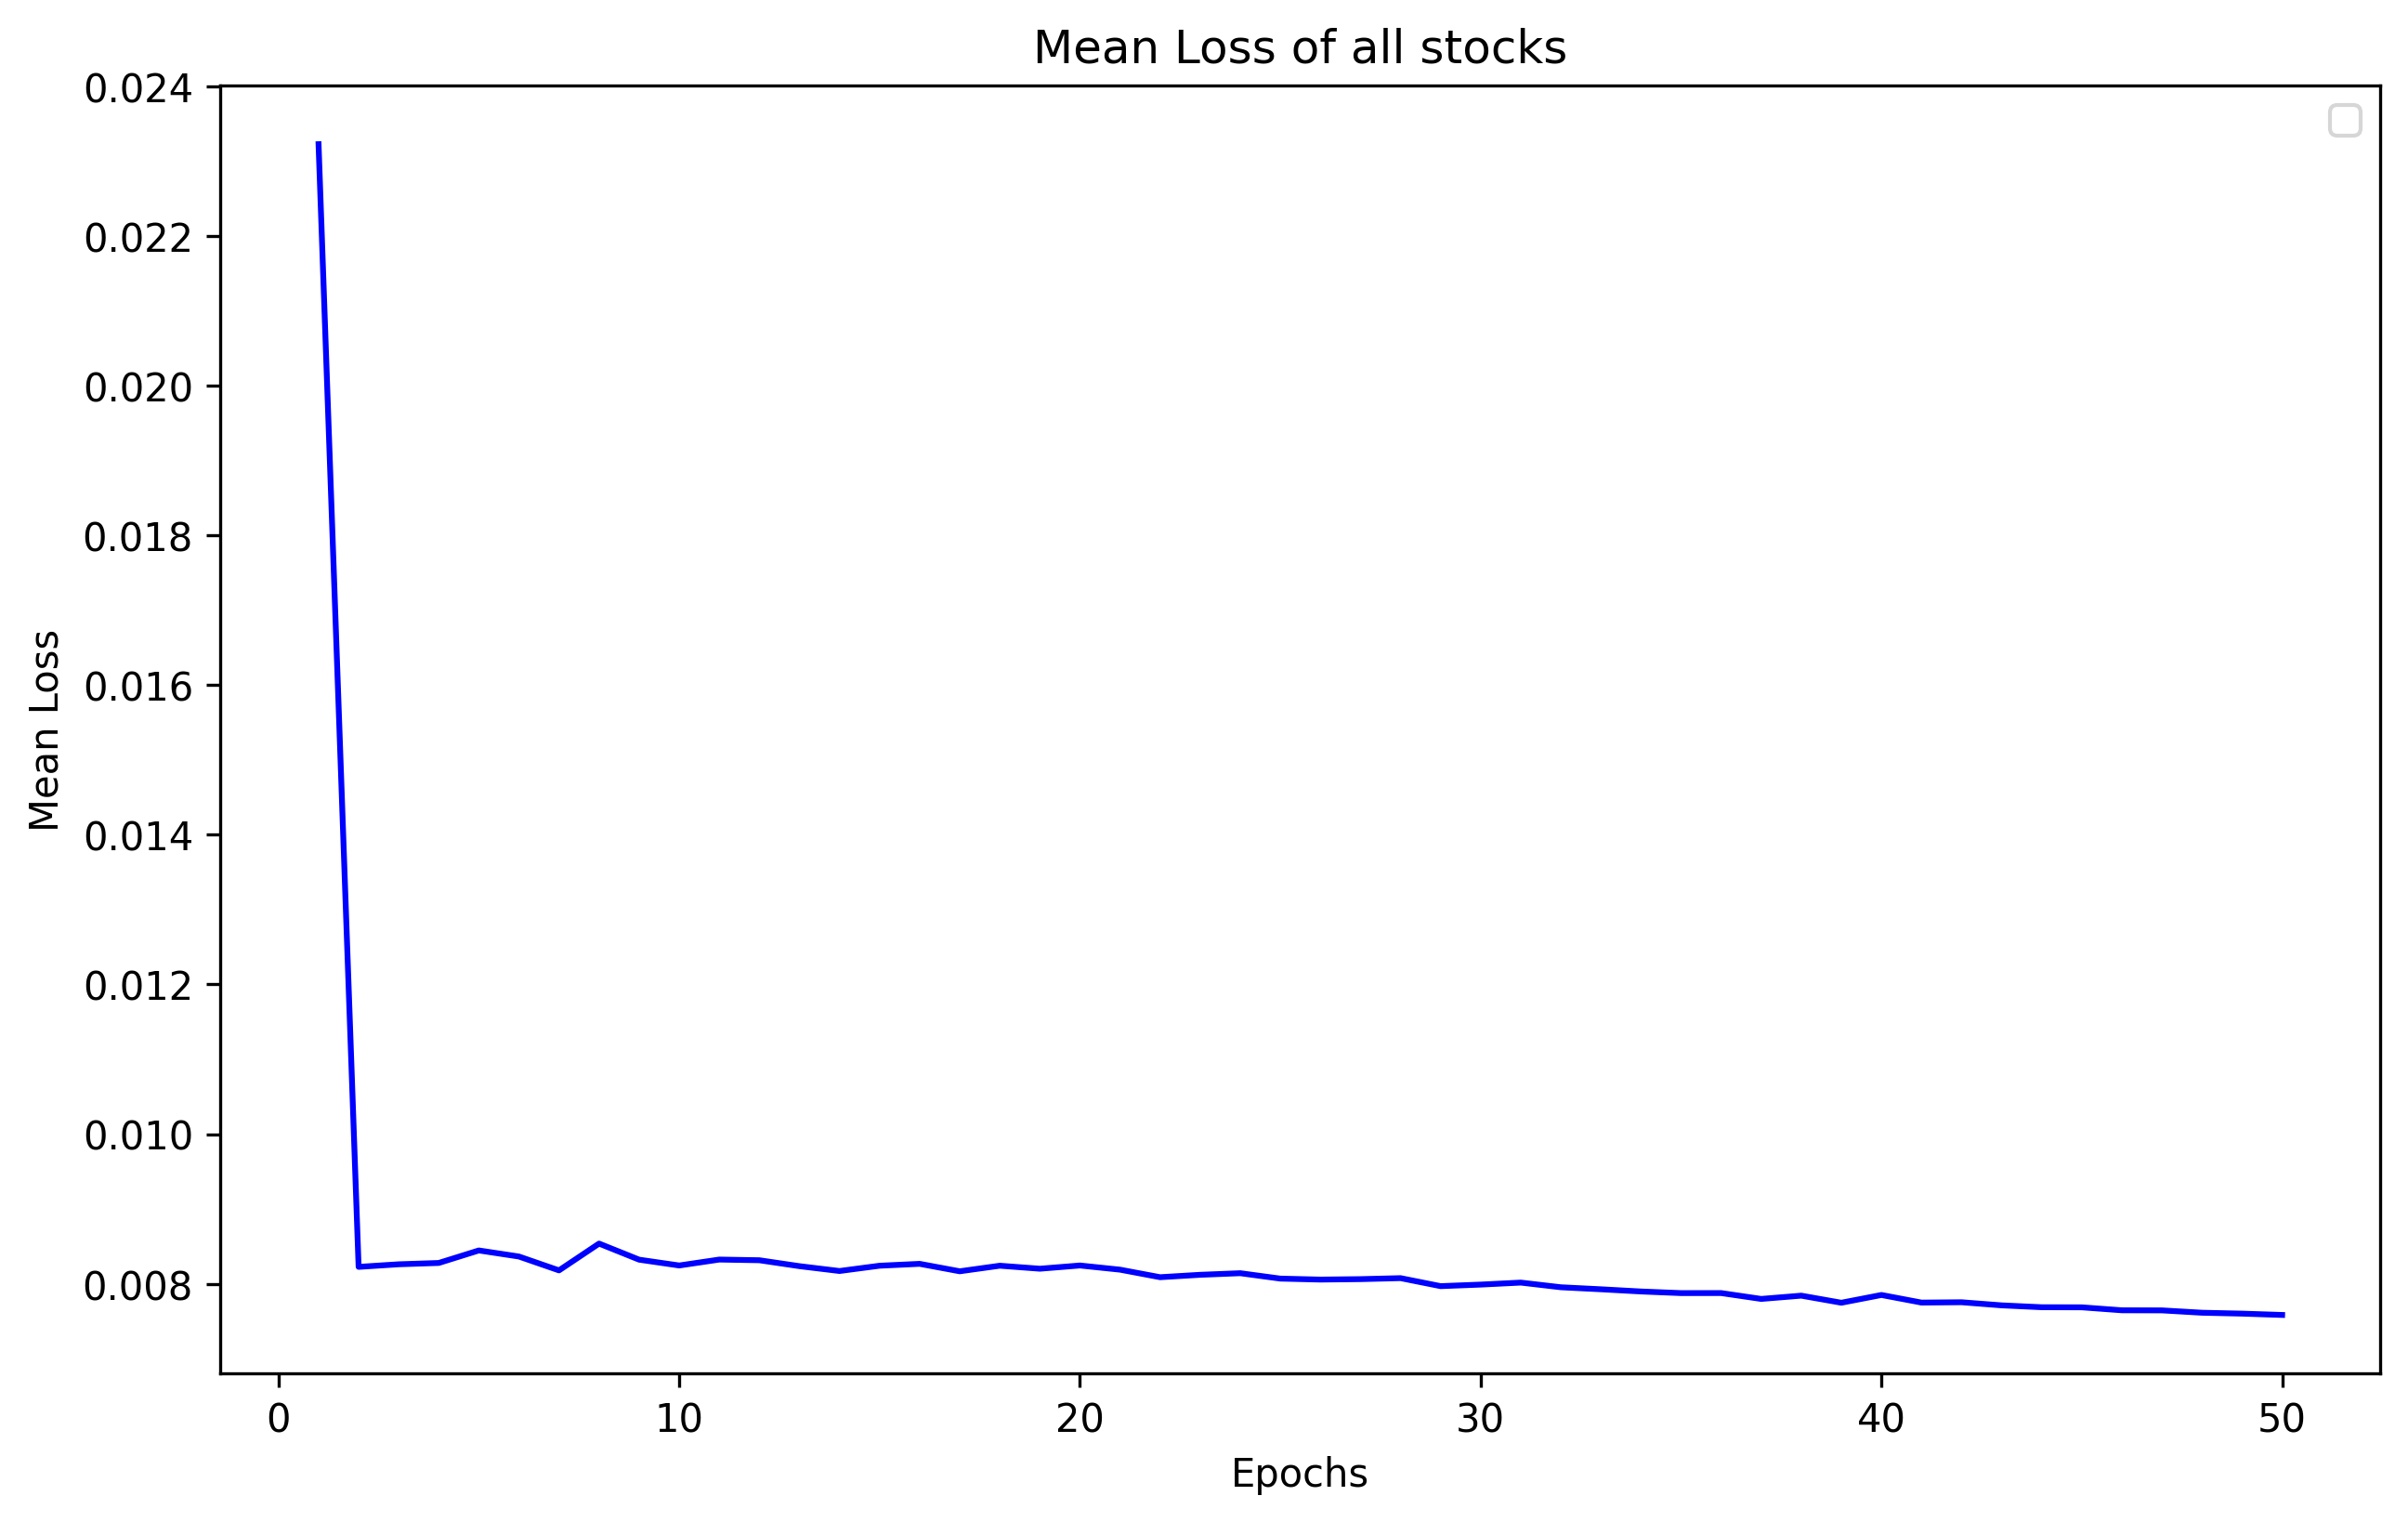
\includegraphics{QCP Report Template/gfx/TrainMeanLoss.png}
  }
 \caption{Mean Loss of all stocks: This plot shows the trend of minimizing the mean loss across all stocks during the training process over 50 epochs. The loss decreases sharply initially and then levels off, indicating the QLSTM model is learning and stabilizing.}
 \label{fig:TrainMeanLoss}
\end{figure}

\subsection{Models' Parameters Comparison}
We have adjusted a few parameters before training our QLSTM model in order to make assumptions on which parameter has what effects on the results. 32 models with slight changes in parameters have been trained and tested throughout the experiment. 

% \begin{figure}[h]
% \centering
%   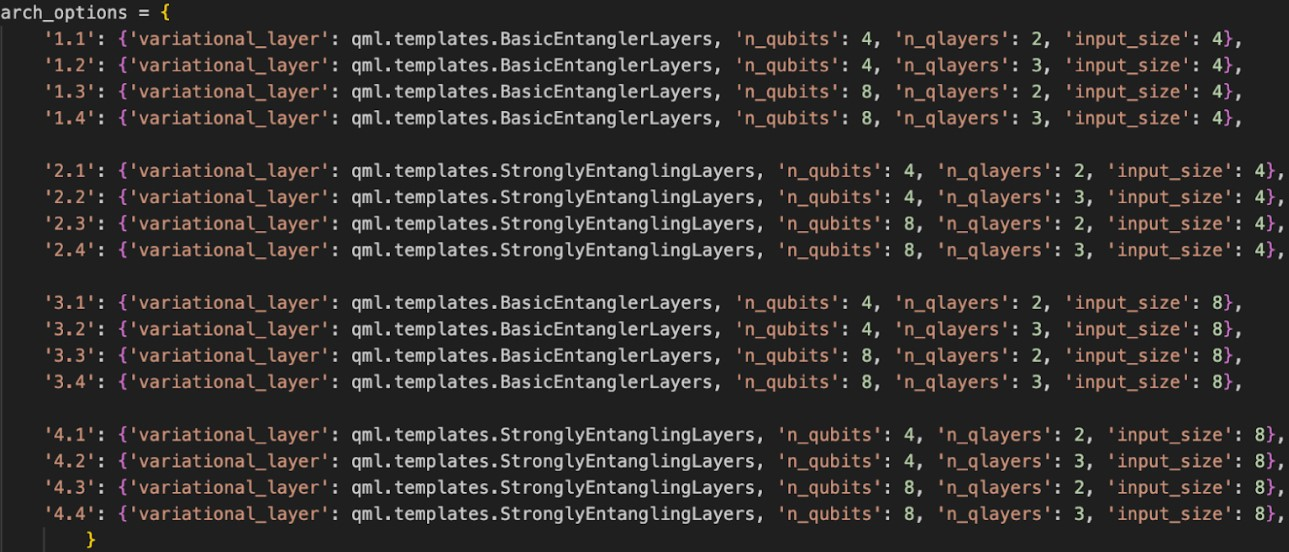
\includegraphics[width=1.0\columnwidth]{gfx/arch_options}
%   \hfill
%  \caption{Model architectures with parameters}
%  \label{fig:Architecture Options}
% \end{figure}

\begin{table}[htbp]
\centering
\label{tab:variational_layers}
\scriptsize
\begin{tabular}{ccccc}
\hline
\textbf{ID} & \textbf{Variational Layer} & \textbf{n\textunderscore Qubits} & \textbf{n\textunderscore Variational Layers} & \textbf{Input Size} \\
\hline
1.1 & BasicEntanglerLayers & 4 & 2 & 4 \\
1.2 & BasicEntanglerLayers & 4 & 3 & 4 \\
1.3 & BasicEntanglerLayers & 8 & 2 & 4 \\
1.4 & BasicEntanglerLayers & 8 & 3 & 4 \\
2.1 & StronglyEntanglingLayers & 4 & 2 & 4 \\
2.2 & StronglyEntanglingLayers & 4 & 3 & 4 \\
2.3 & StronglyEntanglingLayers & 8 & 2 & 4 \\
2.4 & StronglyEntanglingLayers & 8 & 3 & 4 \\
3.1 & BasicEntanglerLayers & 4 & 2 & 8 \\
3.2 & BasicEntanglerLayers & 4 & 3 & 8 \\
3.3 & BasicEntanglerLayers & 8 & 2 & 8 \\
3.4 & BasicEntanglerLayers & 8 & 3 & 8 \\
4.1 & StronglyEntanglingLayers & 4 & 2 & 8 \\
4.2 & StronglyEntanglingLayers & 4 & 3 & 8 \\
4.3 & StronglyEntanglingLayers & 8 & 2 & 8 \\
4.4 & StronglyEntanglingLayers & 8 & 3 & 8 \\
\hline
\end{tabular}
\caption{Variational Layers and their Parameters}
\end{table}

Among the various architectures considered, the 4.2 architecture with a lookback of 5 exhibited the highest mean trend accuracy across all seeds and stocks. This version of the QLSTM model was configured with 4 qubits, 3 variational layers, and 8 input features, utilizing strongly entangling layers. The efficacy of our model is illustrated in Figures~\ref{fig:NFLX}, \ref{fig:PM}, and \ref{fig:TSM}, where it is benchmarked against alternative architectures utilized in our work. Interestingly, although employing 8 input features might intuitively lead to more accurate predictions, the choice of the lookback parameter demonstrated the opposite effect. Most models performed better with a lookback of 5 compared to 10 for one-day predictions, primarily due to the risk of overfitting associated with higher lookback values during training. A similar trend was observed when comparing the number of qubits, where an increase in qubits often resulted in lower-quality predictions.

Additionally, increasing the number of variational layers generally yielded positive effects on the model's performance. However, the difference between 2 and 3 layers did not significantly stand out in the comparison. The subsequent heatmap illustrates how the best-performing model (4.2, lookback 5) on the right side compares to slightly adjusted architectures. The values depicted in the heatmap represent the percentage of correct trend predictions on a specific stock across all 5 seeds.

\begin{figure}[h]
\centering
  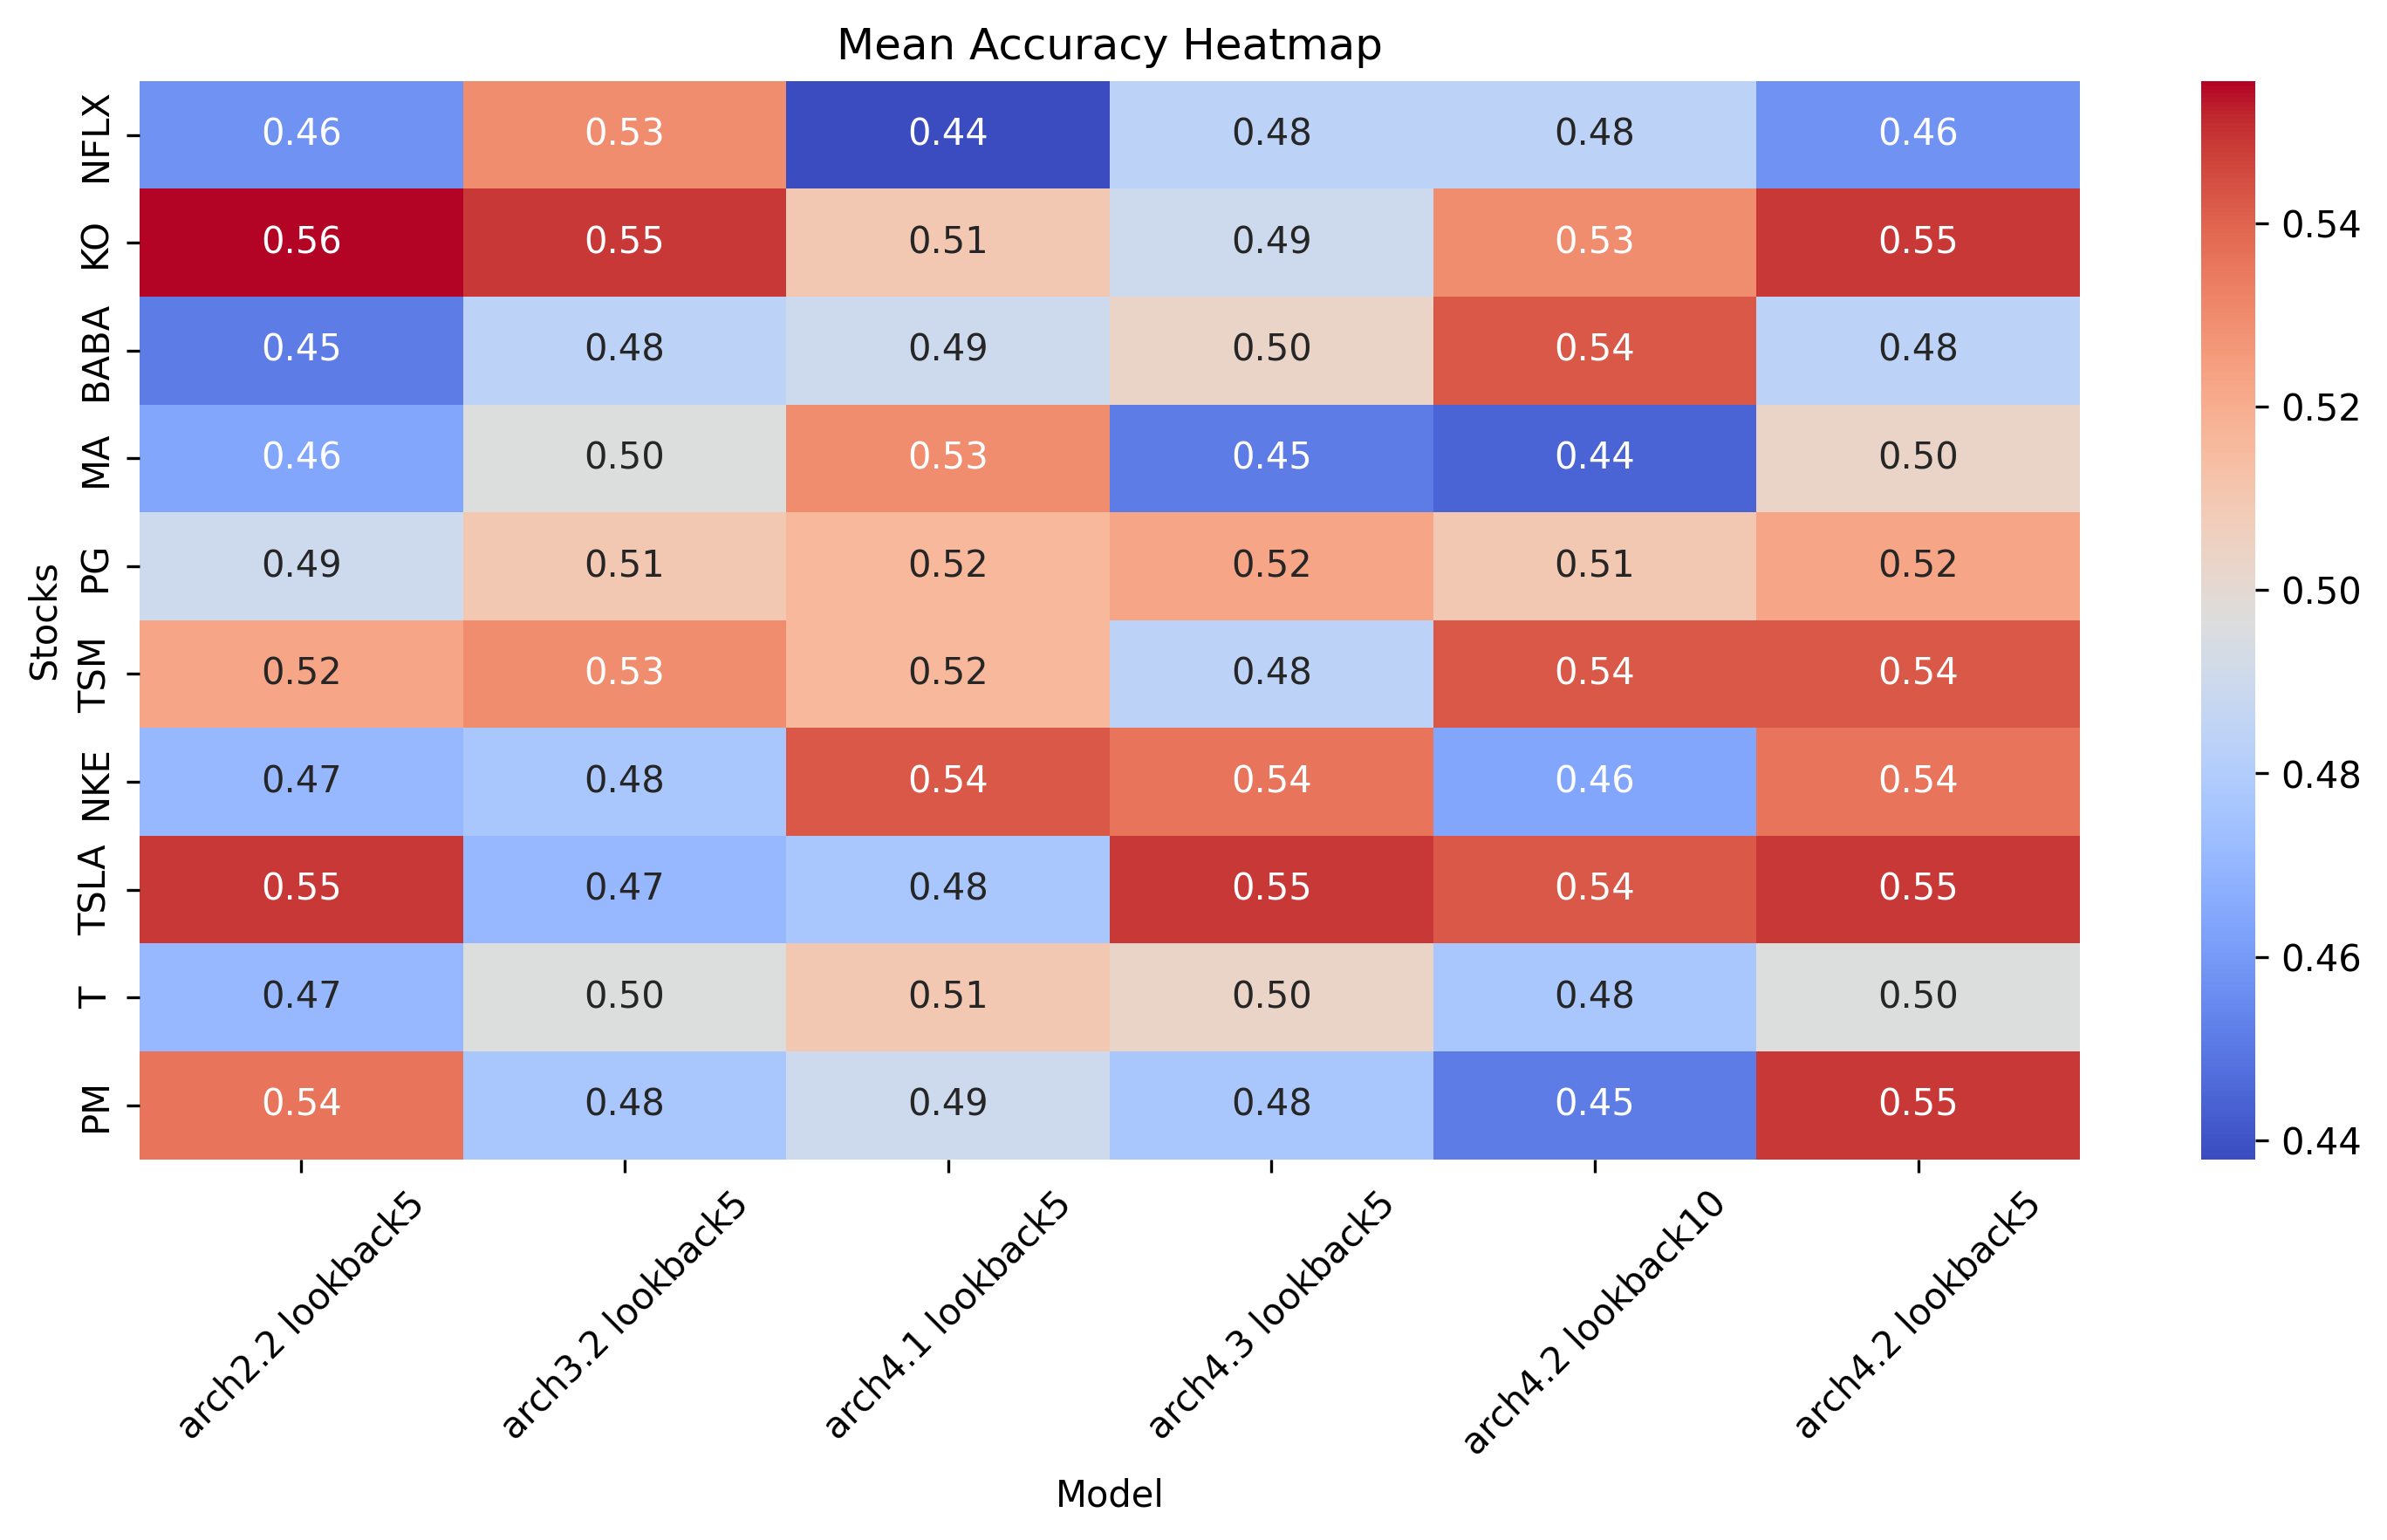
\includegraphics[width=1.0\columnwidth]{gfx/Heatmap}
  \hfill
 \caption{Heatmap with accuracy for different architectures on different stocks}
 \label{fig:Heatmap}
\end{figure}

\begin{figure}[!htbp]
  \centering
  \scalebox{0.30}{
    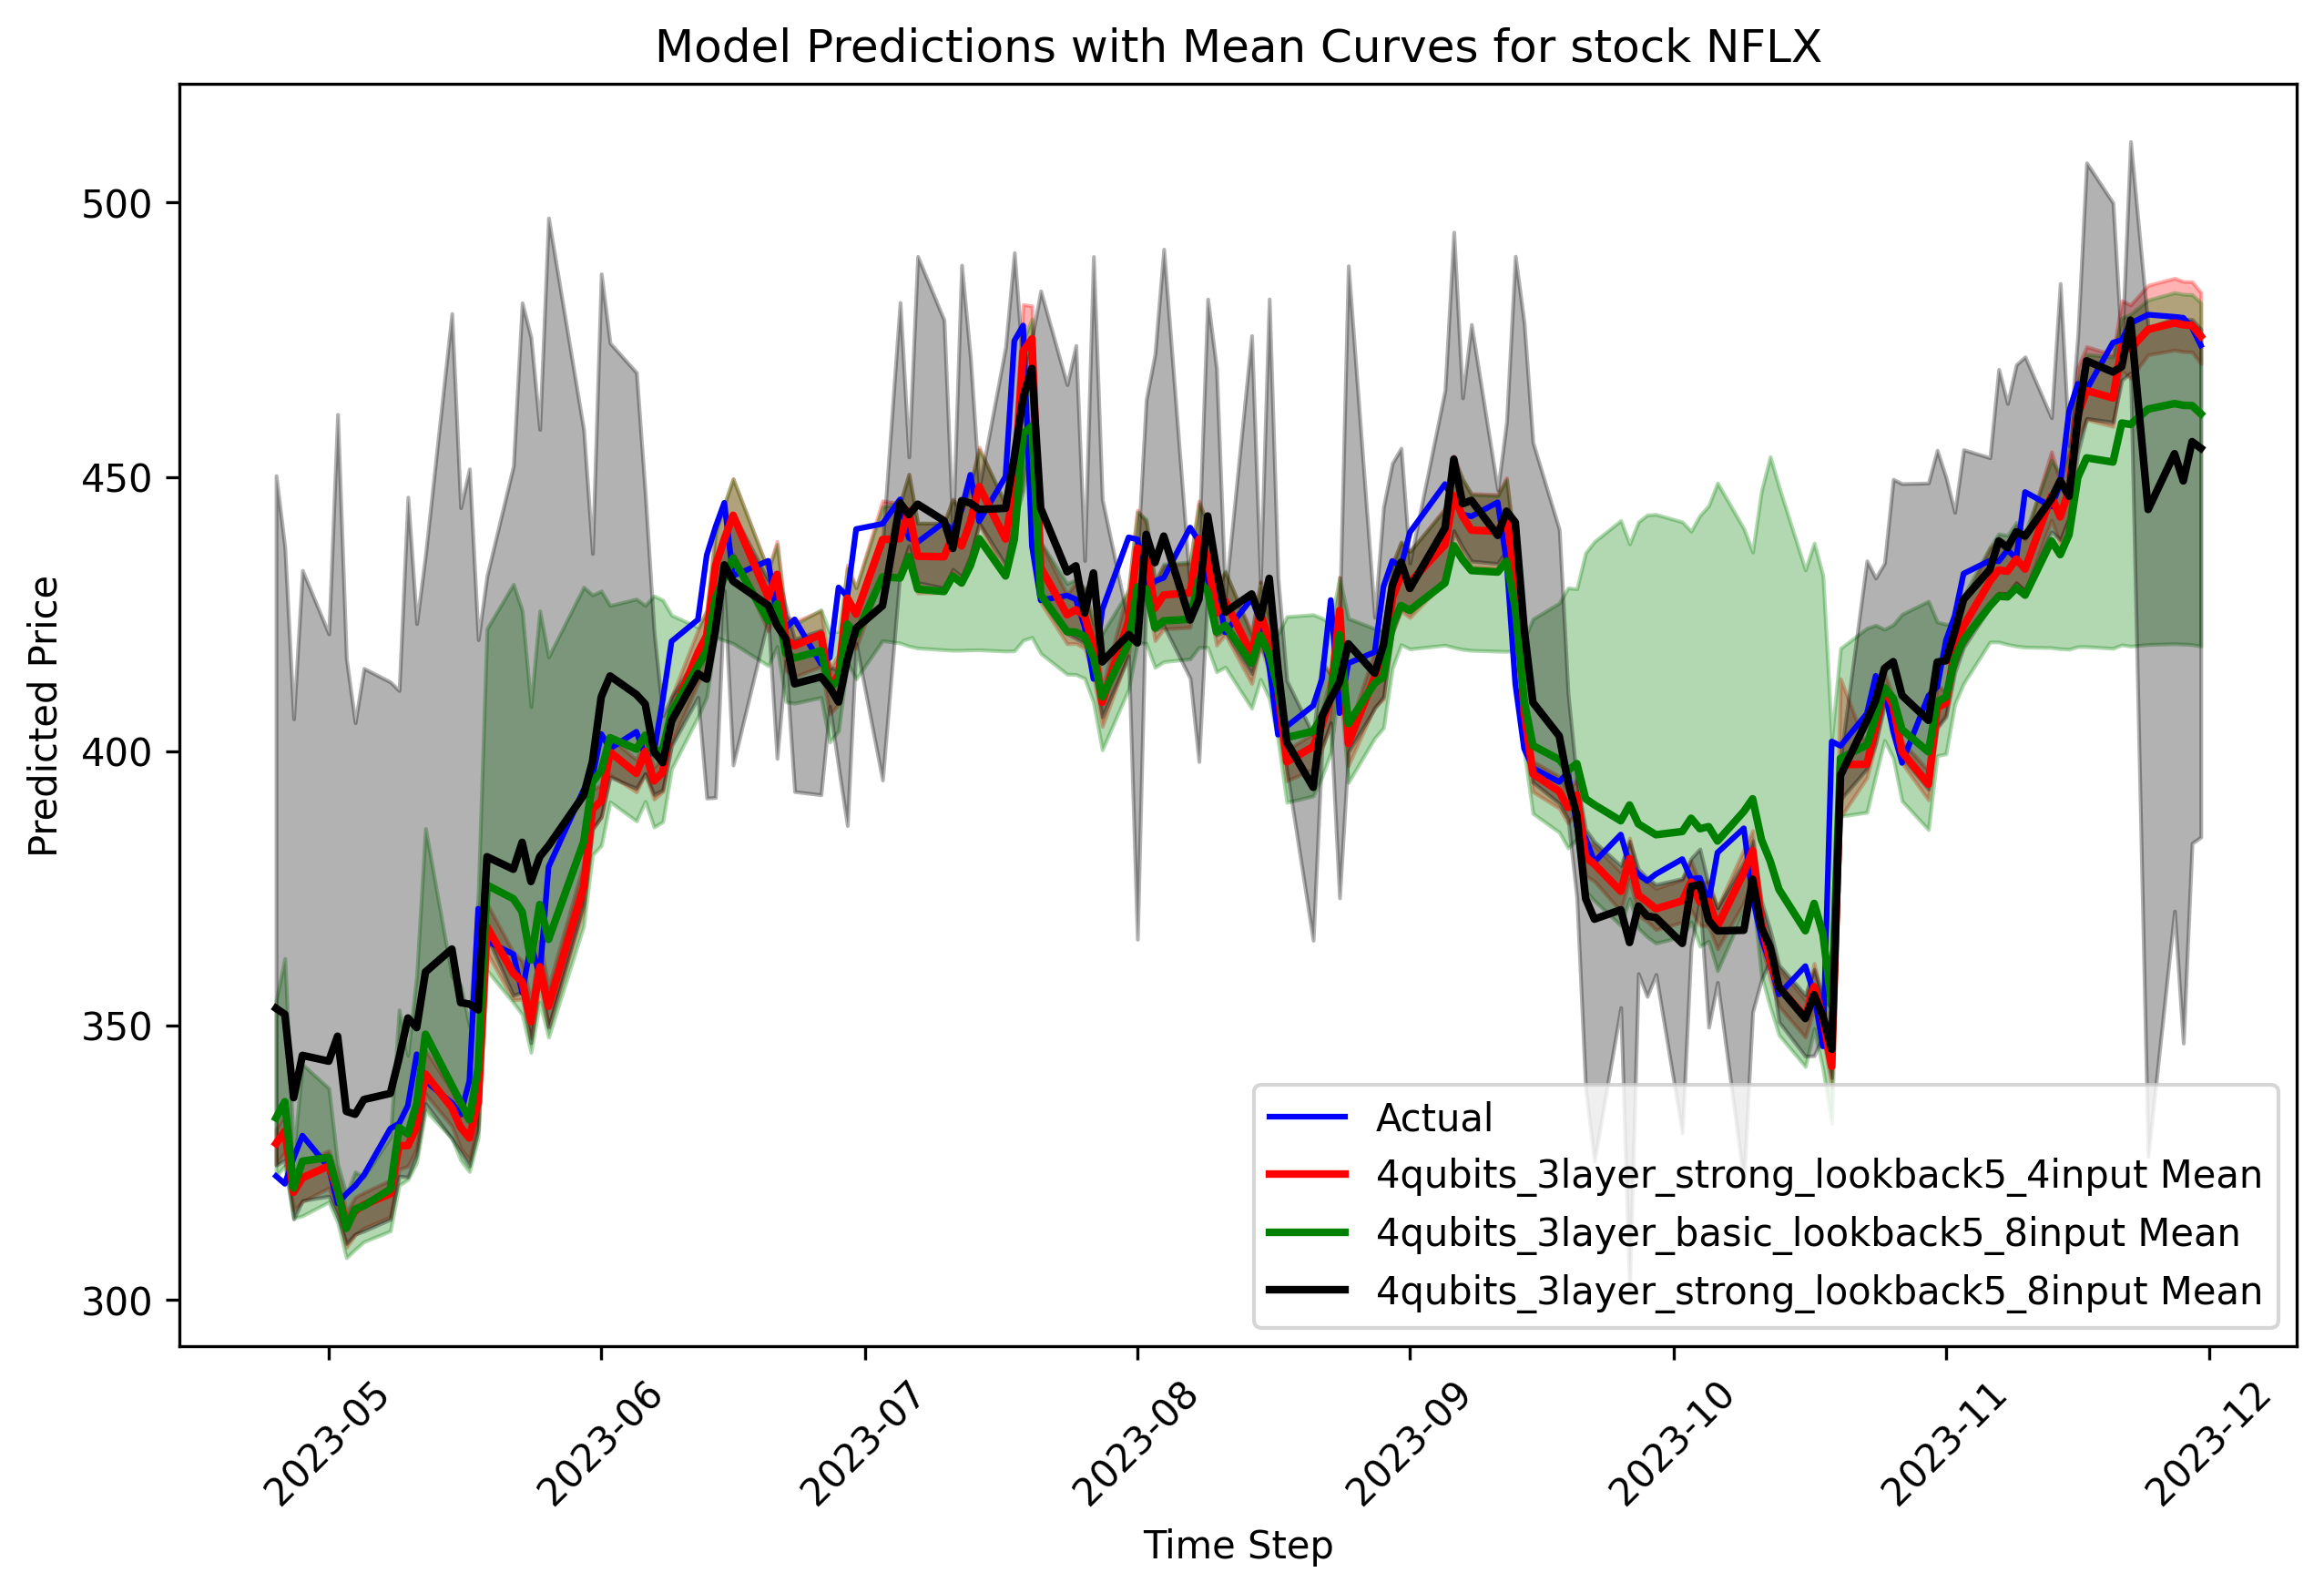
\includegraphics{QCP Report Template/gfx/NFLXMeanCurve.png}
    }
    \caption{Netflix Inc.}
    \label{fig:NFLX}
\end{figure}

\begin{figure}[!htbp]
    \centering
    \scalebox{0.30}{
    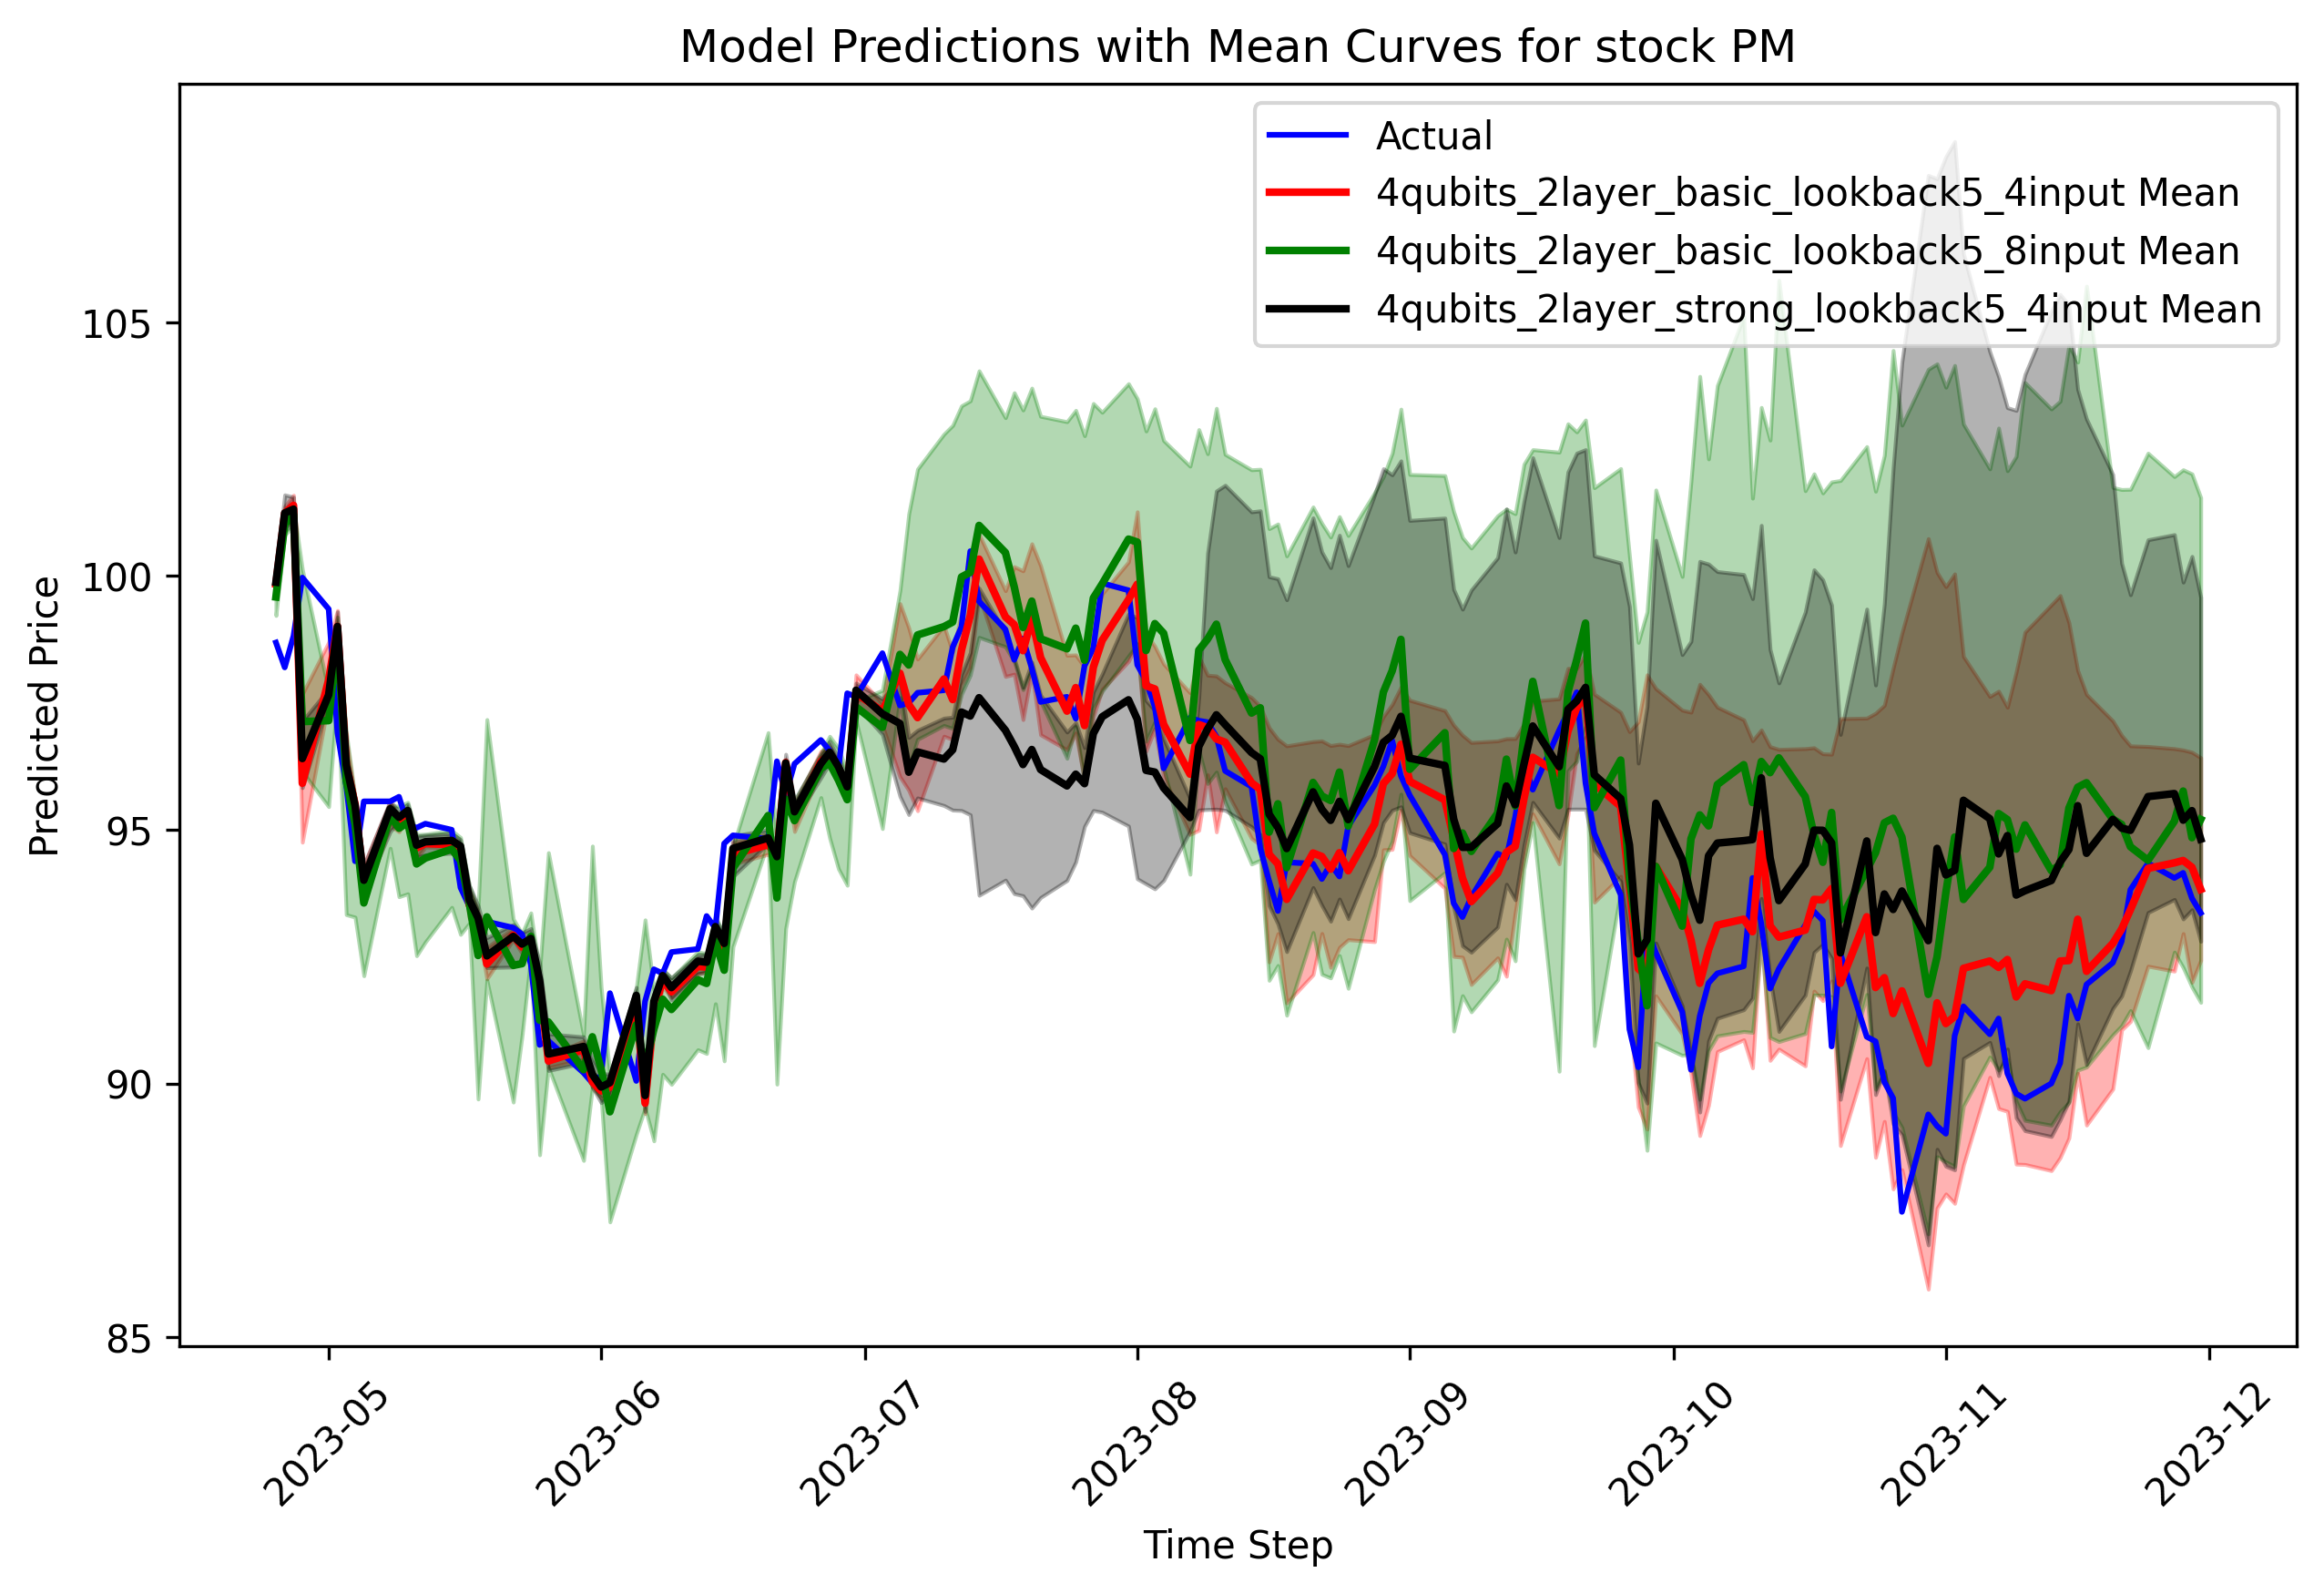
\includegraphics{QCP Report Template/gfx/PMMeanCurve.png}
    }
    \caption{Philip Morris International Inc.} 
    \label{fig:PM}
\end{figure}


\begin{figure}[!htbp]
    \centering
    \scalebox{0.30}{
    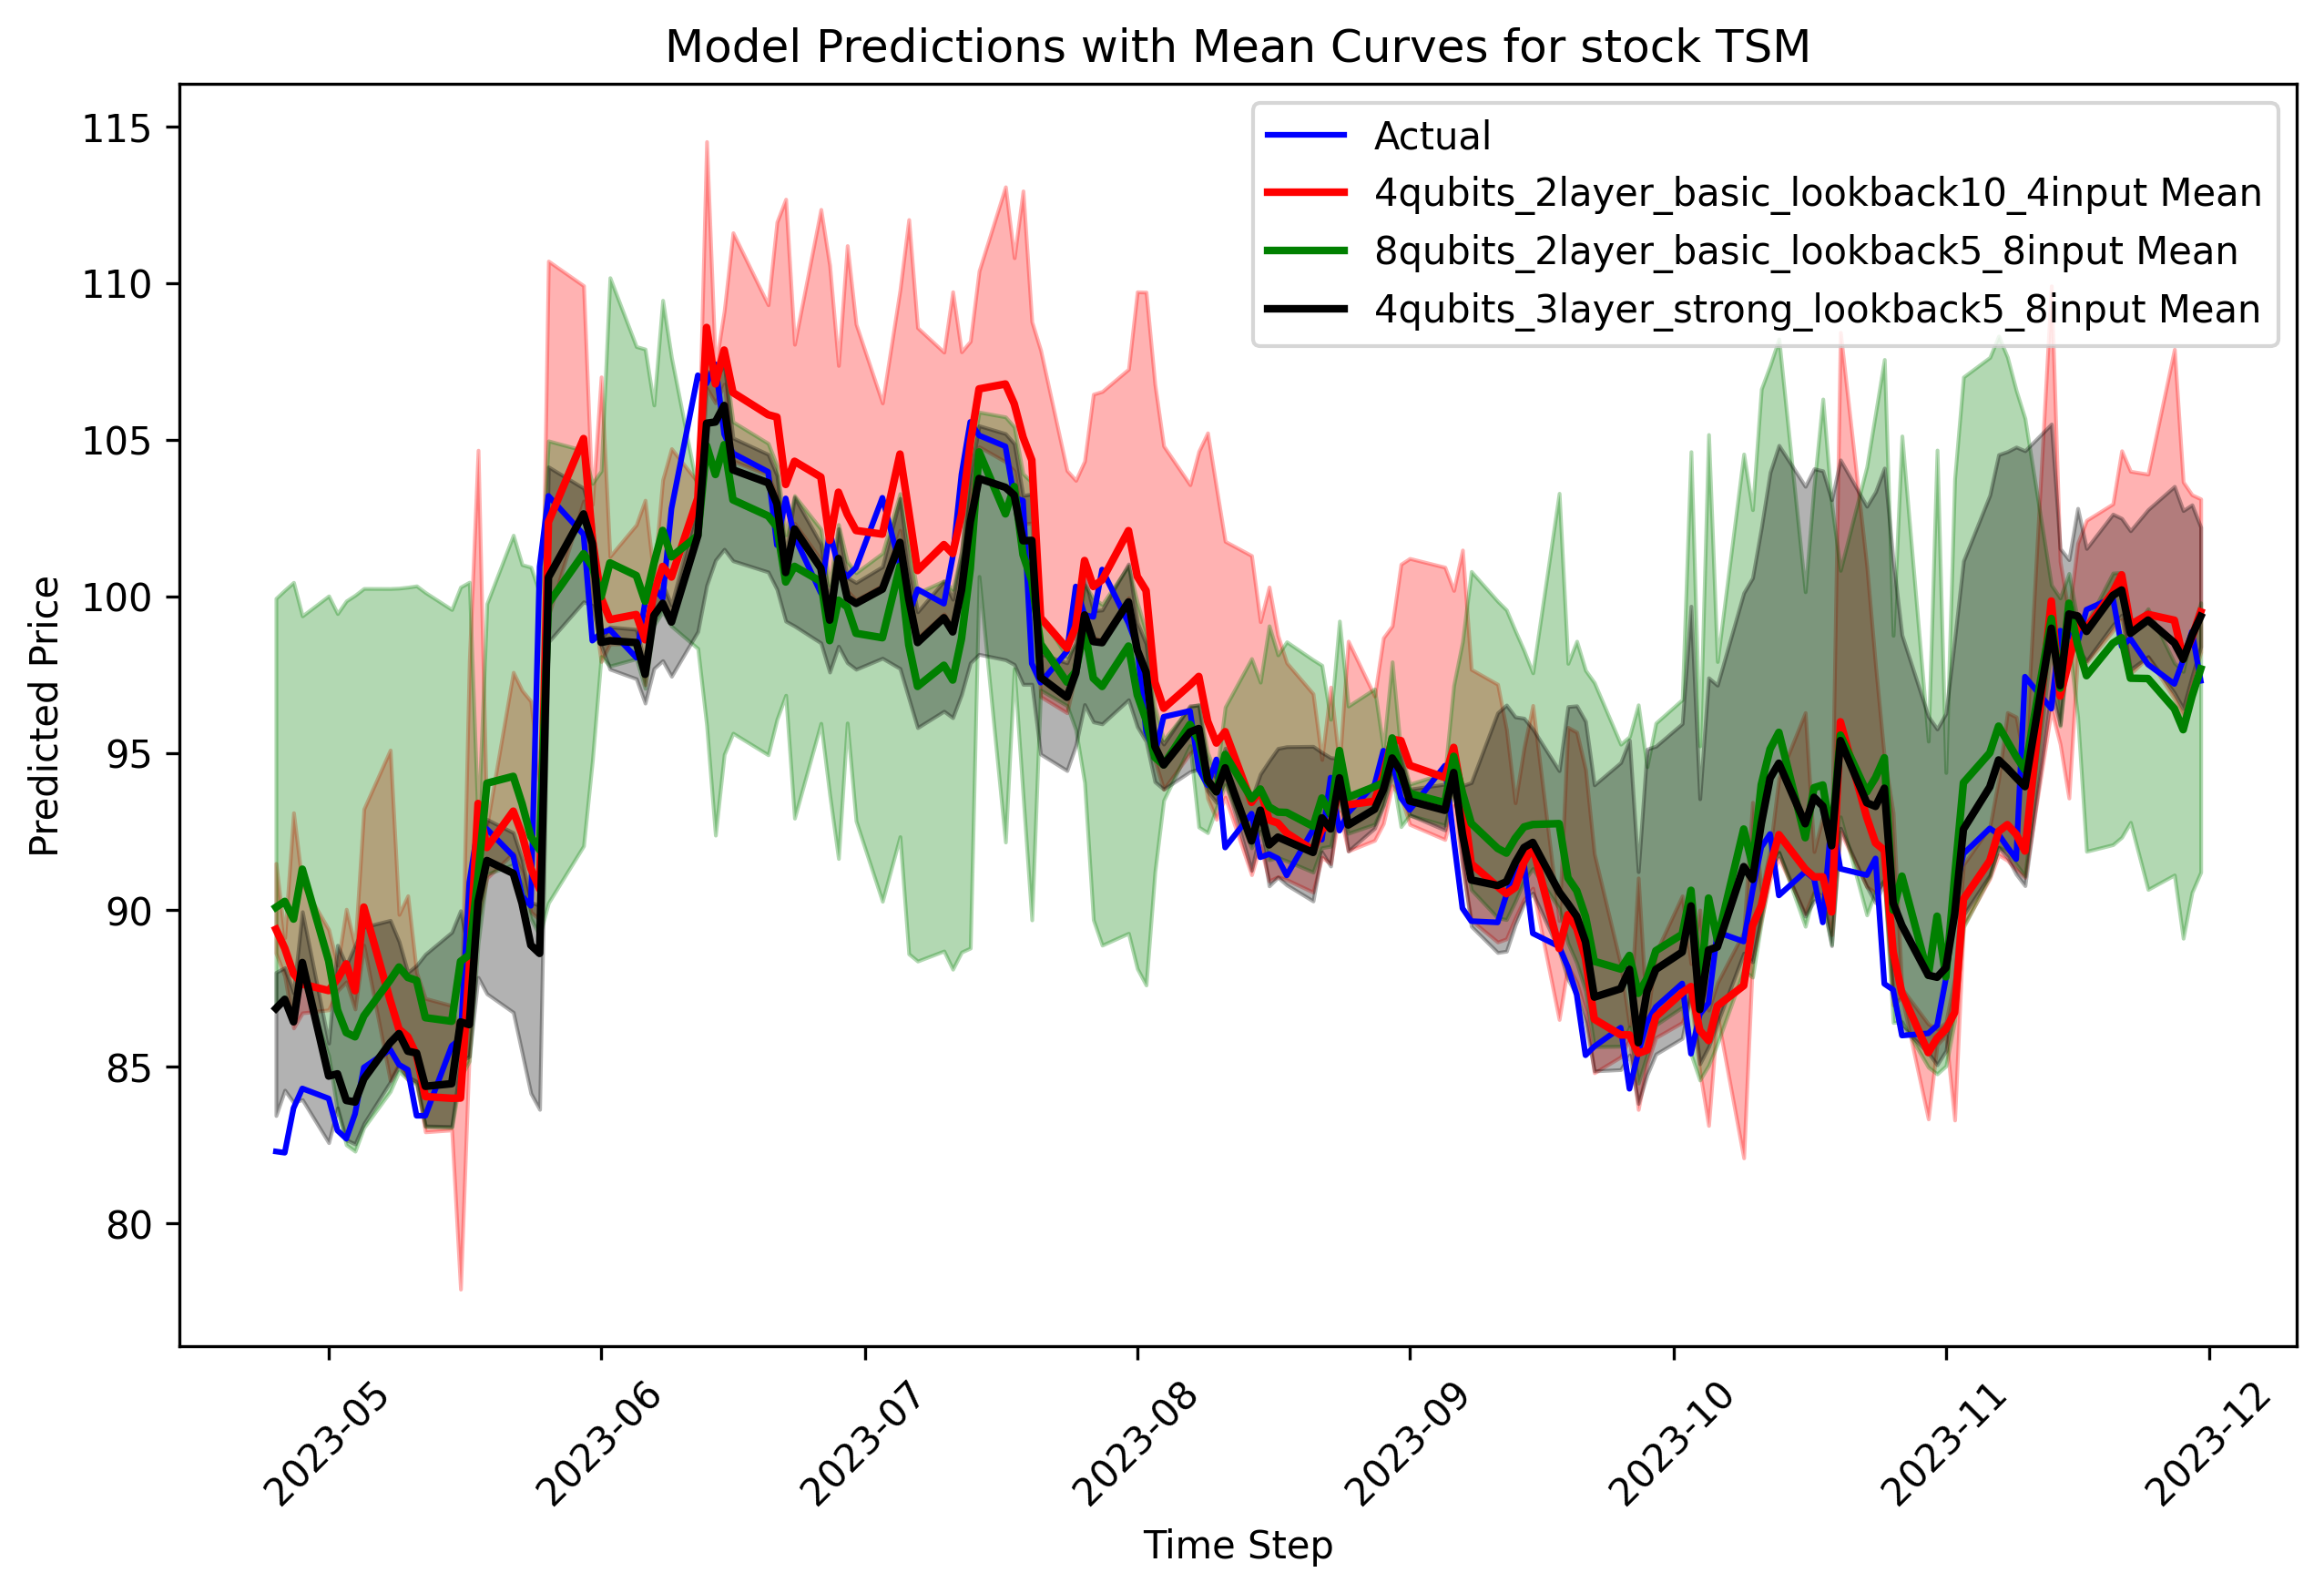
\includegraphics{QCP Report Template/gfx/TSMMeanCurve.png}
    }
    \caption{Taiwan Semiconductor Mfg. Co. Ltd.}
    \label{fig:TSM}
\end{figure}

 
\subsection{Algorithms' Performance for one-day and ten-day Predictions}
We compare our best model (4.2 lookback 5 \ref{tab:variational_layers}) to the QRNN, a classical LSTM and the baseline.
The following plots show the models' predictions of the Philip Morris International Inc. stock as an example \ref{fig:PMPercentReturn}, \ref{fig:PM1day}, \ref{fig:PM10day}.

\begin{figure}[!htbp]
  \centering
  \scalebox{0.30}{
  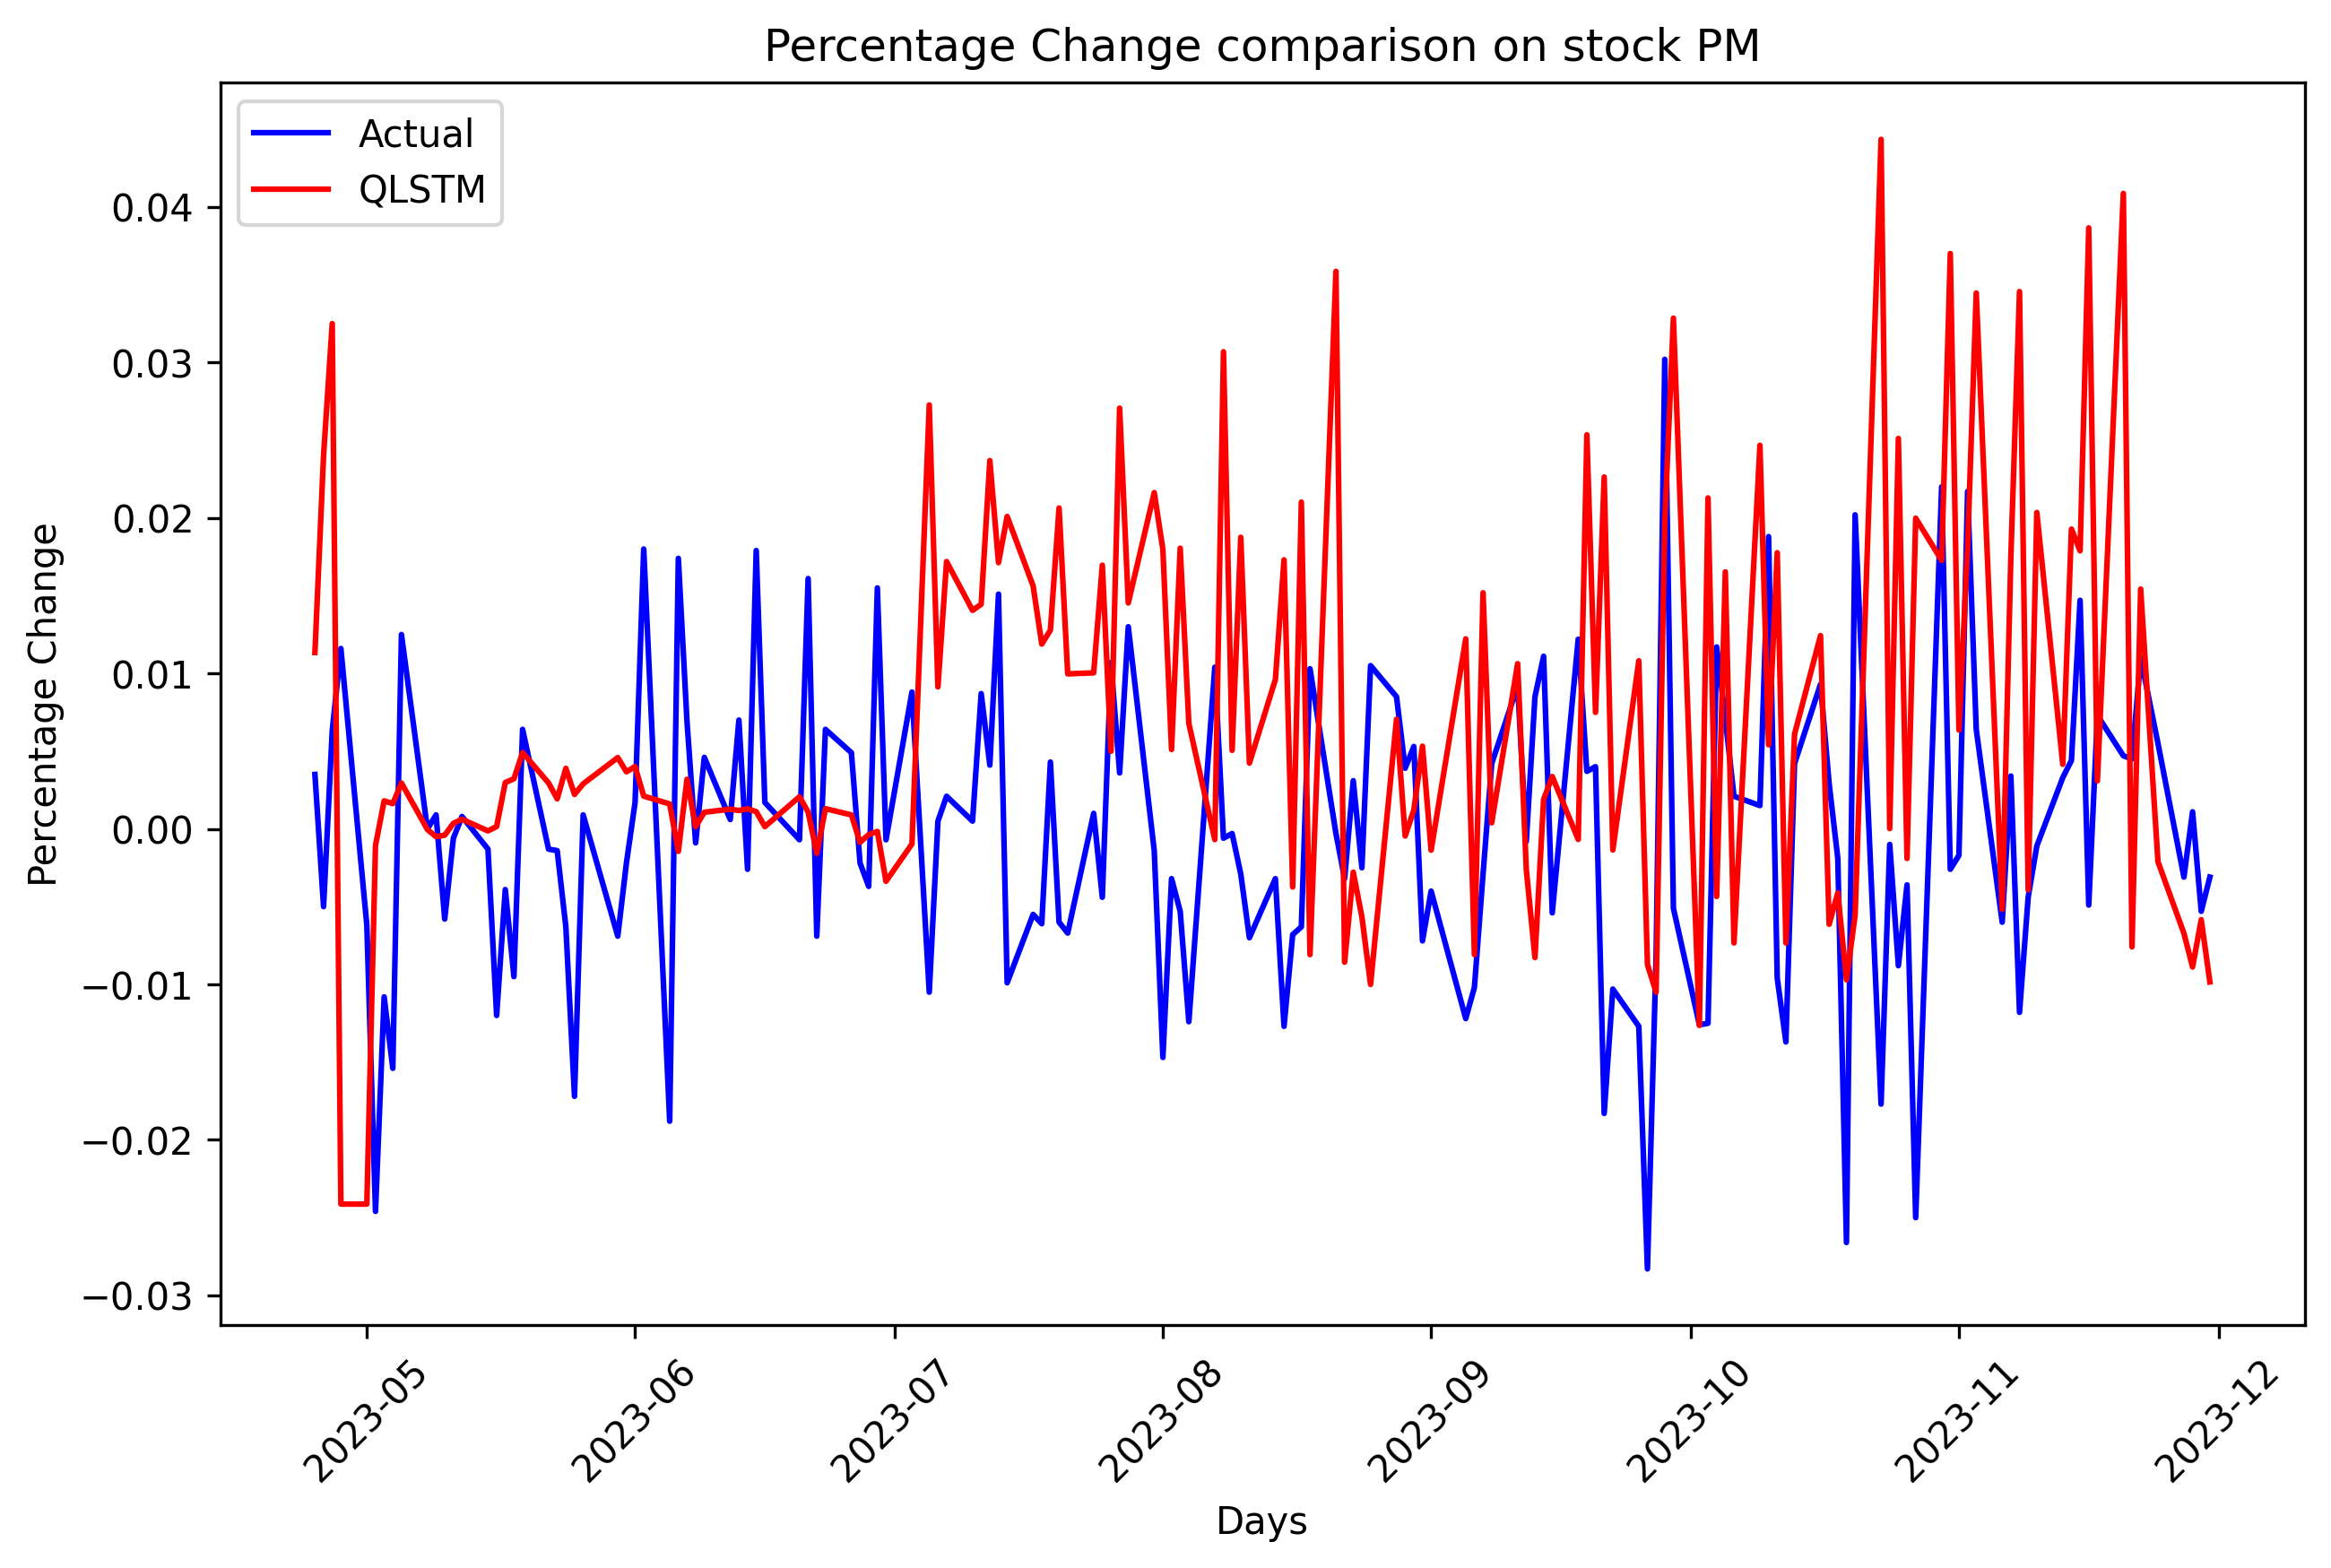
\includegraphics{QCP Report Template/gfx/PMPercentReturn.png}
  }
 \caption{Percentage Change of Philip Morris Stock: A comparison between the actual and QLSTM-predicted percentage change in Philip Morris stock over time.}
 \label{fig:PMPercentReturn}
\end{figure}

\begin{figure}[!htbp]
  \centering
  \scalebox{0.30}{
  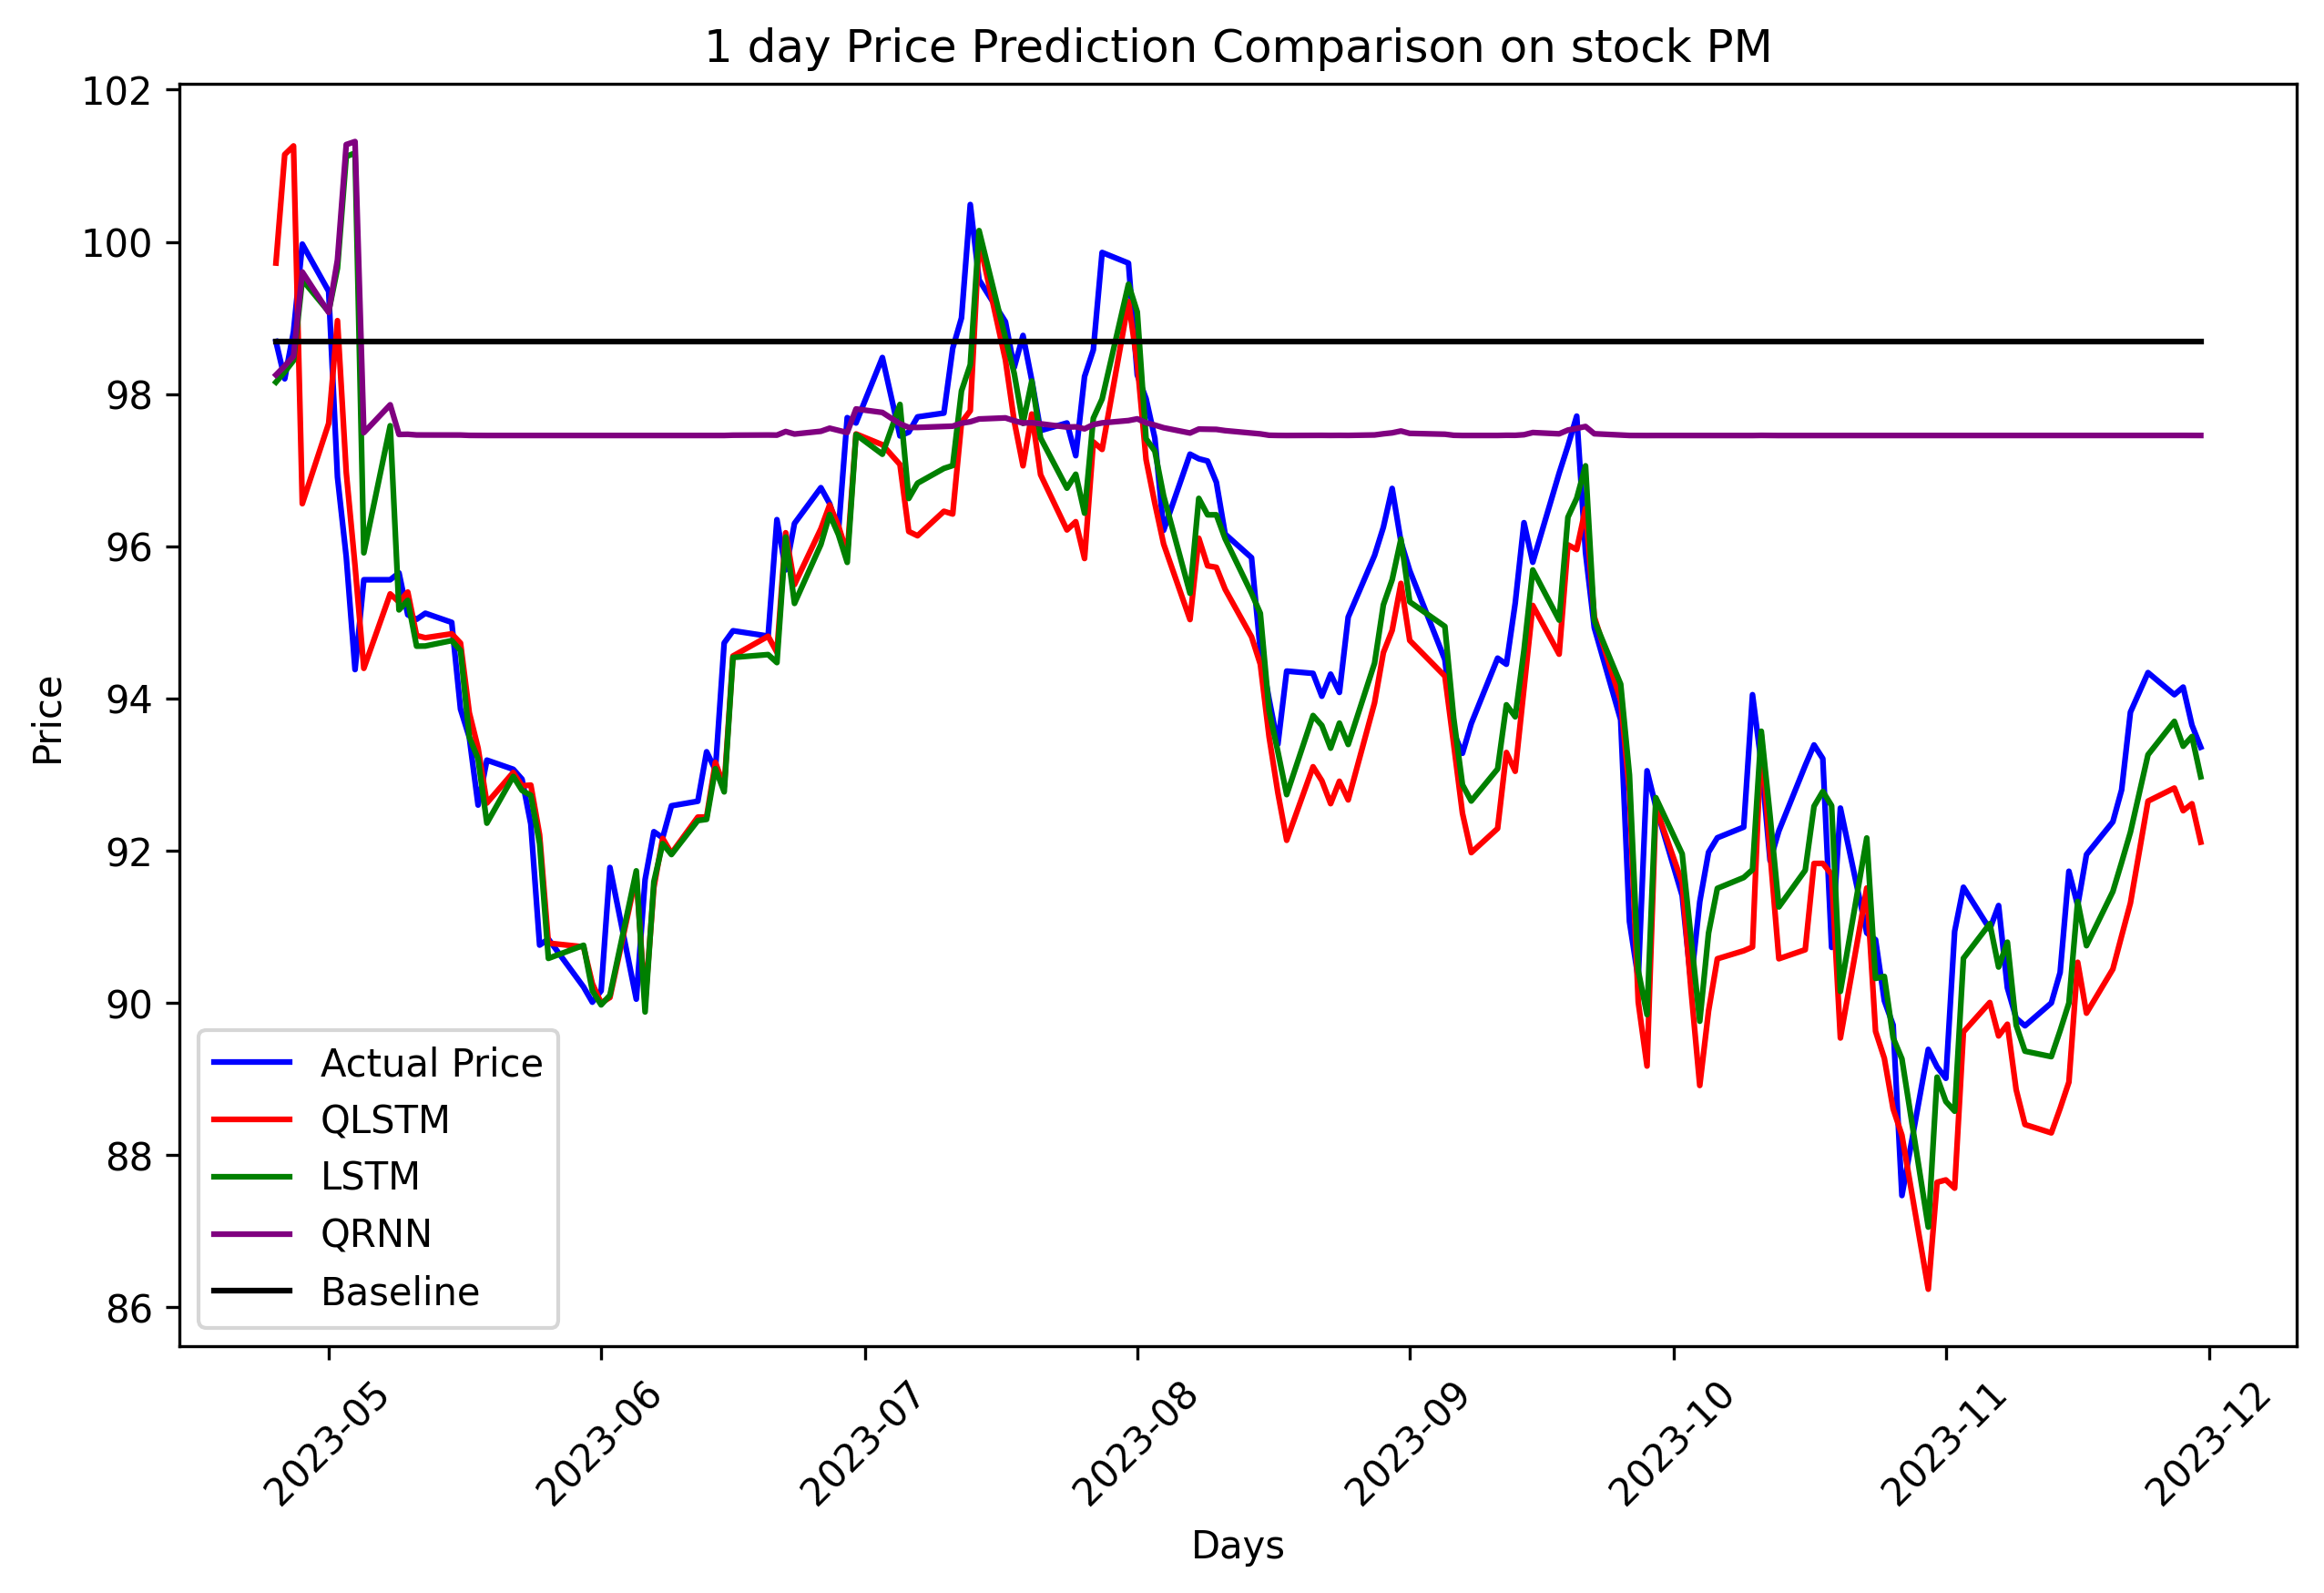
\includegraphics{gfx/PM1day}
  }
 \caption{1-day prediction performance of all the models}
 \label{fig:PM1day}
\end{figure}

\begin{figure}[!htbp]
  \centering
  \scalebox{0.30}{
  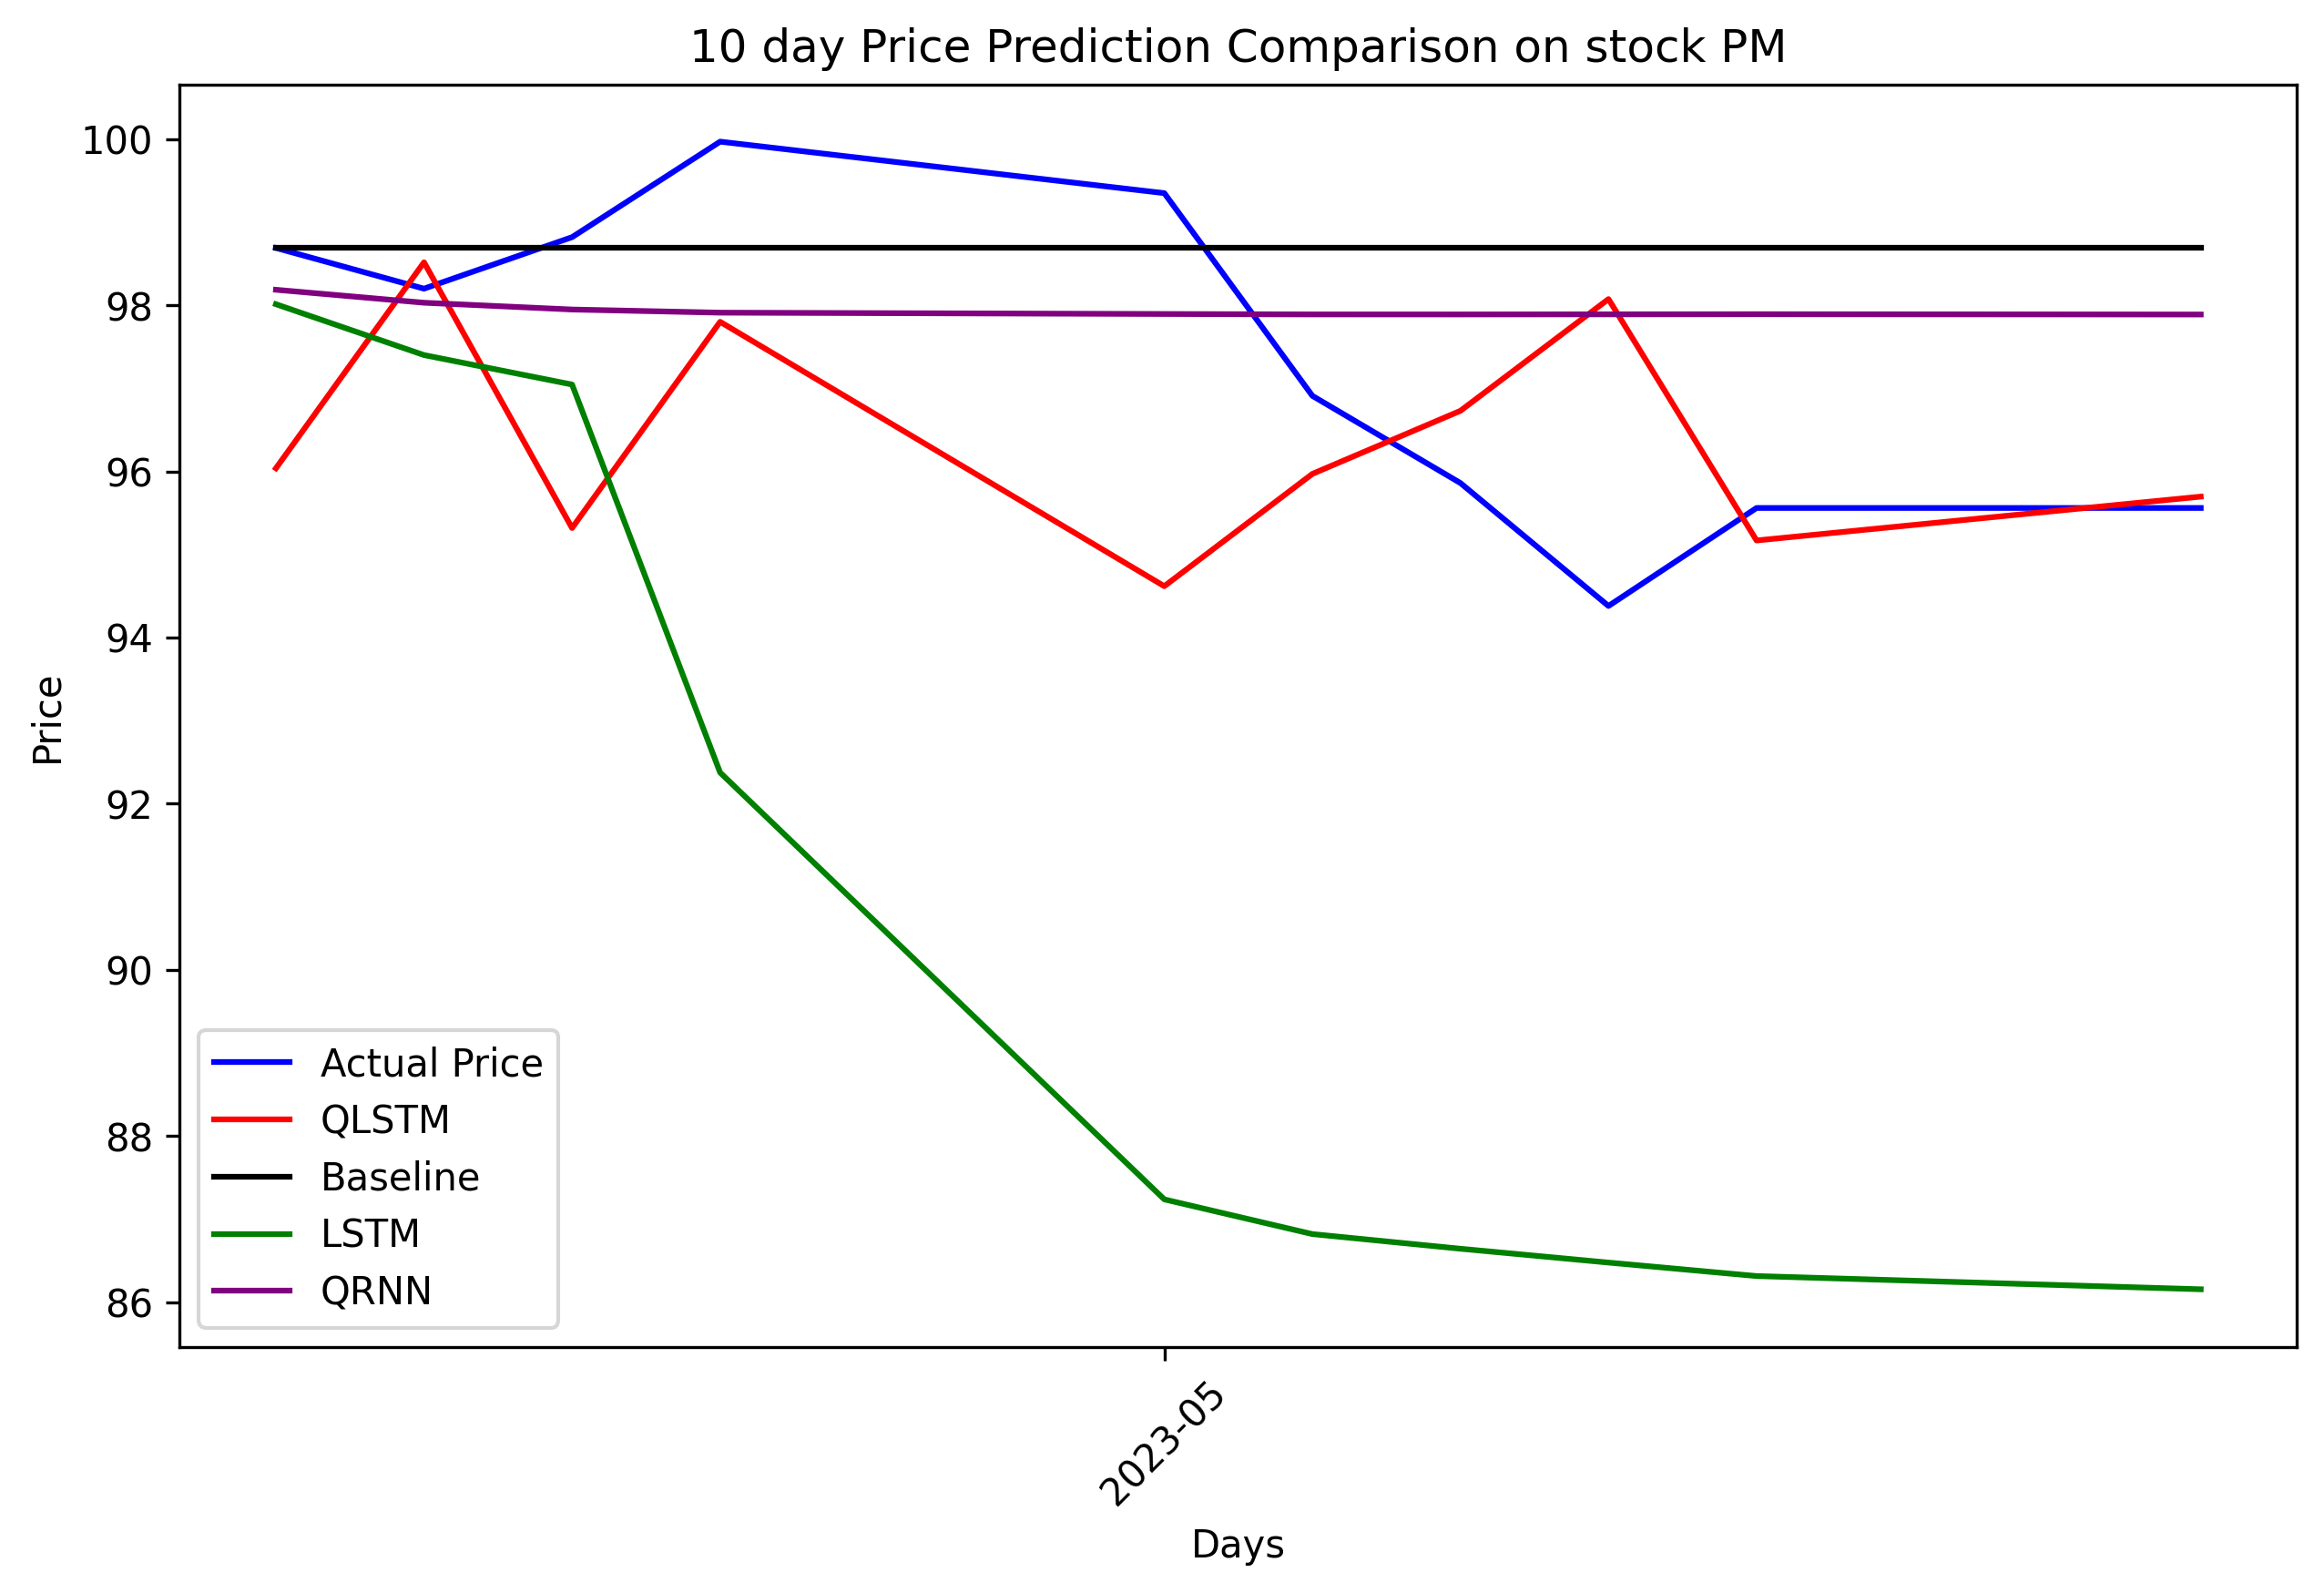
\includegraphics{gfx/PM10day}
  }
 \caption{10-day future prediction performance of all the models}
 \label{fig:PM10day}
\end{figure}

Overall, the QLSTM and classical LSTM networks exhibited comparable performance across all evaluated stocks, achieving a low MSE loss. However, both models achieved an average trend accuracy around 50 percent, indicating that their predictive capability for trend direction does not substantially surpass that of random chance with respect to this metric. Notably, the QLSTM outperformed the LSTM in ten-day forecast horizons, manifesting reduced loss figures. Nevertheless, the LSTM demonstrated a generally similar trend prediction capacity. In contrast, the QRNN and the established baseline model underperformed, incurring higher losses.

